\documentclass[dvipdfmx,uplatex,b5paper,openany,class=gachimuchi]{standalone}
\usepackage{gcmcstyle}
\expandafter\pgfrealjobname\expandafter{\jobname}
\begin{document}
\expandafter\beginpgfgraphicnamed\expandafter{\jobname-fig1}
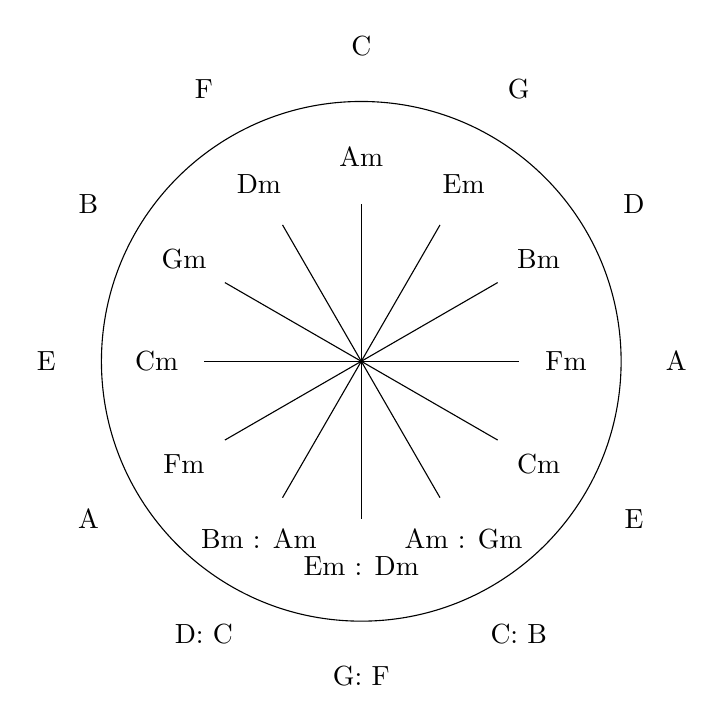
\begin{tikzpicture} % tikzpicture環境開始
\foreach \angle / \label / \Label in
{%
	 90/C/Am, 120/F/Dm, 150/B\aFlat/Gm,
	 180/E\aFlat/Cm, 210/A\aFlat/Fm, 240/D\aFlat : C\aSharp/B\aFlat m : A\aSharp m,
	 270/G\aFlat : F\aSharp/E\aFlat m : D\aSharp m/, 300/C\aFlat : B/A\aFlat m : G\aSharp m/, 330/E/C\aSharp m,
	 0/A/F\aSharp m, 30/D/Bm, 60/G/Em
}
{%
	\draw (\angle:0cm) -- (\angle:2.0cm); 
	\node at (\angle:2.6cm) {\Label};
	\node at (\angle:4.0cm) {\label};
};
\draw (0,0) circle [radius=3.3cm];
\end{tikzpicture} % tikzpicture環境終了
\end{document}
